
%% bare_conf.tex
%% V1.3
%% 2007/01/11
%% by Michael Shell
%% See:
%% http://www.michaelshell.org/
%% for current contact information.
%%
%% This is a skeleton file demonstrating the use of IEEEtran.cls
%% (requires IEEEtran.cls version 1.7 or later) with an IEEE conference paper.
%%
%% Support sites:
%% http://www.michaelshell.org/tex/ieeetran/
%% http://www.ctan.org/tex-archive/macros/latex/contrib/IEEEtran/
%% and
%% http://www.ieee.org/

%%*************************************************************************
%% Legal Notice:
%% This code is offered as-is without any warranty either expressed or
%% implied; without even the implied warranty of MERCHANTABILITY or
%% FITNESS FOR A PARTICULAR PURPOSE! 
%% User assumes all risk.
%% In no event shall IEEE or any contributor to this code be liable for
%% any damages or losses, including, but not limited to, incidental,
%% consequential, or any other damages, resulting from the use or misuse
%% of any information contained here.
%%
%% All comments are the opinions of their respective authors and are not
%% necessarily endorsed by the IEEE.
%%
%% This work is distributed under the LaTeX Project Public License (LPPL)
%% ( http://www.latex-project.org/ ) version 1.3, and may be freely used,
%% distributed and modified. A copy of the LPPL, version 1.3, is included
%% in the base LaTeX documentation of all distributions of LaTeX released
%% 2003/12/01 or later.
%% Retain all contribution notices and credits.
%% ** Modified files should be clearly indicated as such, including  **
%% ** renaming them and changing author support contact information. **
%%
%% File list of work: IEEEtran.cls, IEEEtran_HOWTO.pdf, bare_adv.tex,
%%                    bare_conf.tex, bare_jrnl.tex, bare_jrnl_compsoc.tex
%%*************************************************************************

% *** Authors should verify (and, if needed, correct) their LaTeX system  ***
% *** with the testflow diagnostic prior to trusting their LaTeX platform ***
% *** with production work. IEEE's font choices can trigger bugs that do  ***
% *** not appear when using other class files.                            ***
% The testflow support page is at:
% http://www.michaelshell.org/tex/testflow/



% Note that the a4paper option is mainly intended so that authors in
% countries using A4 can easily print to A4 and see how their papers will
% look in print - the typesetting of the document will not typically be
% affected with changes in paper size (but the bottom and side margins will).
% Use the testflow package mentioned above to verify correct handling of
% both paper sizes by the user's LaTeX system.
%
% Also note that the "draftcls" or "draftclsnofoot", not "draft", option
% should be used if it is desired that the figures are to be displayed in
% draft mode.
%
% \documentclass[11pt,conference]{IEEEtran}

\documentclass[11pt]{article}
\usepackage{geometry}
 \geometry{
 a4paper,
 left=0.75in,
 right=0.75in,
 top=0in,
 bottom=0in
 }
%\usepackage{ifpdf}
% Heiko Oberdiek's ifpdf.sty is very useful if you need conditional
% compilation based on whether the output is pdf or dvi.
% usage:
% \ifpdf
%   % pdf code
% \else
%   % dvi code
% \fi
% The latest version of ifpdf.sty can be obtained from:
% http://www.ctan.org/tex-archive/macros/latex/contrib/oberdiek/
% Also, note that IEEEtran.cls V1.7 and later provides a builtin
% \ifCLASSINFOpdf conditional that works the same way.
% When switching from latex to pdflatex and vice-versa, the compiler may
% have to be run twice to clear warning/error messages.

\usepackage{cite}
% cite.sty was written by Donald Arseneau
% V1.6 and later of IEEEtran pre-defines the format of the cite.sty package
% \cite{} output to follow that of IEEE. Loading the cite package will
% result in citation numbers being automatically sorted and properly
% "compressed/ranged". e.g., [1], [9], [2], [7], [5], [6] without using
% cite.sty will become [1], [2], [5]--[7], [9] using cite.sty. cite.sty's
% \cite will automatically add leading space, if needed. Use cite.sty's
% noadjust option (cite.sty V3.8 and later) if you want to turn this off.
% cite.sty is already installed on most LaTeX systems. Be sure and use
% version 4.0 (2003-05-27) and later if using hyperref.sty. cite.sty does
% not currently provide for hyperlinked citations.
% The latest version can be obtained at:
% http://www.ctan.org/tex-archive/macros/latex/contrib/cite/
% The documentation is contained in the cite.sty file itself.

\pagenumbering{gobble} 
\usepackage{float}
\usepackage[cmex10]{amsmath}
\usepackage{amsmath}
\usepackage{macros}
\usepackage{mathtools}
\usepackage{algorithmic}
\usepackage{array}
\usepackage{mdwmath}
\usepackage{mdwtab}
\usepackage{eqparbox}
% \usepackage[tight,footnotesize]{subfigure}
\usepackage[caption=false]{caption}
\usepackage[font=footnotesize]{subfig}
\usepackage{stfloats}
\usepackage{url}
\usepackage{bbm}
\usepackage{tikz-cd}
\usepackage{flowchart}
\usepackage{tabularx}
\usepackage{array}
\DeclareMathOperator{\Cech}{\check{C}}
% correct bad hyphenation here
\hyphenation{op-tical net-works semi-conduc-tor}
% Use the Palatino font by default
\usepackage{booktabs}
\usepackage{colortbl}
\usepackage{hyperref}
\date{}
\begin{document}
%
% paper title
% can use linebreaks \\ within to get better formatting as desired
\title{Comparing neural population responses based on pairwise $p$-Wasserstein distance between topological signatures}


% author names and affiliations
% use a multiple column layout for up to three different
% affiliations
% \author{\IEEEauthorblockN{Anonymous authors}}

% conference papers do not typically use \thanks and this command
% is locked out in conference mode. If really needed, such as for
% the acknowledgment of grants, issue a \IEEEoverridecommandlockouts
% after \documentclass

% for over three affiliations, or if they all won't fit within the width
% of the page, use this alternative format:
% 
%\author{\IEEEauthorblockN{Michael Shell\IEEEauthorrefmark{1},
%Homer Simpson\IEEEauthorrefmark{2},
%James Kirk\IEEEauthorrefmark{3}, 
%Montgomery Scott\IEEEauthorrefmark{3} and
%Eldon Tyrell\IEEEauthorrefmark{4}}
%\IEEEauthorblockA{\IEEEauthorrefmark{1}School of Electrical and Computer Engineering\\
%Georgia Institute of Technology,
%Atlanta, Georgia 30332--0250\\ Email: see http://www.michaelshell.org/contact.html}
%\IEEEauthorblockA{\IEEEauthorrefmark{2}Twentieth Century Fox, Springfield, USA\\
%Email: homer@thesimpsons.com}
%\IEEEauthorblockA{\IEEEauthorrefmark{3}Starfleet Academy, San Francisco, California 96678-2391\\
%Telephone: (800) 555--1212, Fax: (888) 555--1212}
%\IEEEauthorblockA{\IEEEauthorrefmark{4}Tyrell Inc., 123 Replicant Street, Los Angeles, California 90210--4321}}


% use for special paper notices
%\IEEEspecialpapernotice{(Invited Paper)}


% make the title area
\maketitle
\vspace{-0.6in}
% For peer review papers, you can put extra information on the cover
% page as needed:
% \ifCLASSOPTIONpeerreview
% \begin{center} \bfseries EDICS Category: 3-BBND \end{center}
% \fi
%
% For peerreview papers, this IEEEtran command inserts a page break and
% creates the second title. It will be ignored for other modes.
% \IEEEpeerreviewmaketitle
Real-world data are often encoded in high-dimensional representations. Moreover, it is often unclear which coordinates and metrics can be meaningfully justified. Topological properties are well-suited for characterizing the structure of such high-dimensional data point-cloud: they are generalized to high-dimensional surfaces; they are also invariant under different coordinates and robust to the choice of metrics. Our work aims to compare data point-clouds in terms of their topological properties and is specifically motivated by a recently emerged class of open problems in neuroscience to analyze the high-dimensional output of a population of neurons in response to respective stimuli (hence known as the “neural population response”). Several recent works have successfully applied topology for such problems. However, a crucial gap in these works is that they have not considered how these high-dimensional neural population responses can be appropriately compared, which is key to understanding neural representations.

Our proposed topology-based approach allows a quantitative comparison between neural population responses arising from artificial and biological neural networks. It also allows statistical inference on a distribution of topological signatures for the respective neural population responses. As a demonstration, we apply the approach to compare neural population responses in the mouse retina to different visual stimuli. First, we use nonlinear dimensionality reduction to obtain a lower-dimensional neural manifold. Topological features are then extracted using persistent homology and represented as persistence diagrams. Finally, we compute the pairwise $p$-Wasserstein distance between these persistence diagrams. 
% \section{Introduction}
% Real-world data are often encoded in high-dimensional representations. Moreover, it is often unclear which coordinates and metrics can be meaningfully justified. Topological properties are well-suited for characterizing the structure of such high-dimensional data point-cloud: they are generalized to high-dimensional surfaces; they are also invariant under different coordinates and robust to the choice of metrics. The proposed approach aims to compare data point-clouds in terms of their topological properties and is motivated by a recently emerged class of open problems in neuroscience to analyze the high-dimensional output of a population of neurons in response to respective stimuli (hence known as the “neural population response”). Topology is a promising mathematical tool, but it is rarely used  until a few very recent works. However, a crucial gap in these works is that they have not considered how these high-dimensional neural population responses can be appropriately compared, which is key to understanding neural representations.
% \begin{defn}[Simplicial complex]
% An \underline{abstract simplicial complex} is a pair $(V, \triangle)$, where $V$ is a finite set, and $\triangle$ is a family of non-empty subsets of $V$ such that $\tau \in \triangle \text{ and }\sigma \subseteq \tau \implies \sigma \in \triangle,$ where $\tau \in \triangle $ is face of $\triangle$. The dimension of a face $\tau$ is $|\tau| - 1.$ 
% % ($0$-dimensional faces are vertices. $1$-dimensional faces are edges. A simplicial complex of dimension $D \le 1$ is a simple and loopless graph.)
% \end{defn}

% \begin{defn}[$k$-th homology group]
% \label{kth-homology-group}
% Define the $\mathbb{F}$-module $Z_k(\triangle; \mathbb{F})$ of cycles and the $\FF$-module of he boundary group $B_k(\triangle;\FF)$ by the following formulas:
%     \begin{itemize}
%         \item $Z_k(\triangle; \mathbb{F}) = ker(\partial_k) = \{Z \in \Chain_k(\triangle; \FF): \partial_k(Z) = 0\}$ 
%         \item $B_k(\triangle;\FF) = im(\partial_{k+1}) = \{Z \in \Chain_k(\triangle; \FF): \partial_{k+1}(x), \quad x \in \Chain_{k+1}(\triangle; \FF)\}$ 
%     \end{itemize}
%   \underline{Simplicial homology in degree $k$ of $\triangle$} is the quotient group $\Hom_k(\triangle;\FF) = ker(\partial_k) / im(\partial_{k+1}) = Z_k(\triangle;\FF) / B_k(\triangle;\FF)$.

% % (Intuition) Homology associates a vector space $H_k(X)$ to a topological space $X$ for each $k\in \NN$.
% % \begin{itemize}
% %     \item $H_0(X)$ is the number of path components in $X$.
% %     \item $H_1(X)$ is the number of holes in X.
% %     \item $H_2(X)$ is the number of voids in X.
% % \end{itemize}
% \end{defn}

% \begin{defn}[Filtered simplicial complex]
% \label{filtered}
% A subcomplex of $\triangle$ is a subset $\triangle^i \subseteq \triangle$ that is also a simplicial complex. 
% Let $\triangle$ be a finite simplicial complex and let $\triangle^1 \subset \triangle^2 \subset \cdots \subset \triangle^m = \triangle$ be a finite sequence of nested subcomplexes of $\triangle$. The simplicial complex $\triangle$ with such a sequence of subcomplexes, $\emptyset \subseteq \triangle^1 \subseteq \triangle^2 \subseteq \cdots \subseteq \triangle^m = \triangle$, is called \underline{filtered simplicial complex}.

% % A \underline{filtration} on a simplicial complex $X$ is a collection of subcomplexes $\{X(t) \ |\ t\in \RR\}$ of $X$ such that $X(t) \subset X(t')$ whenever $t\le t'$. The filtration value of a simplex $\sigma \in \triangle$ is the smallest $i$ such that $\sigma \in \triangle^i$. 
% \end{defn}

% \begin{defn}[$p$-persistent $k$-th homology group]
% Given a filtered complex, for the $i$-th subcomplex $\triangle^i$ we compute the associated boundary maps $\partial_k^i$ for all dimensions $k$, boundary matrices $M_k^i$ for all dimensions $k$, $C_k^i, Z_k^i$ (cycle group), $B_k^i$ (boundary group), and $H_k^i$ (homology group). Then the \underline{$p$-persistent $k$-th homology group} $H_k^{i,p}$ of $\triangle^i$ is $Z_k^i / (B_k^{i+p}\cap Z_k^i)$.
%     % \item (equivalently) $H_k{i,p} \cong Im(\eta_k^{i,p})$, where $\eta_k^{i,p}$ is a bijection $\eta_k^{i,p}: H_k^i \to H_k^{i+p}$ that maps a homology class into another homology class containing it.   
% % Note that this is simply the definition of homology group of degree $k$ in Definition \ref{kth-homology-group} with the additional notion of persistence. The main idea of \textit{persistence} is that instead of selecting a fixed value of the threshold $\epsilon$, we would like to obtain a useful summary of the homological information for all the different values of $\epsilon$ at once. As $\epsilon$ increases, we add simplicies to the complexes and detect which features "persist."
% \end{defn}

% \begin{thm}[Barcode and persistent diagrams]
% The rank of $H_k^{i\to j}(\mathscr{C}; F)$ gives the number of intervals in the \underline{barcode} of $H_k^{i\to j}(\mathscr{C}; F)$ spanning the parameter interval $[i,j]$ ($i, j$ represent the ``birth" and ``death" of a feature respectively). \underline{Persistent diagram} is an equivalent representation of barcode, with x-axis and y-axis representing the ``birth" and ``death" of a feature respectively.
% \end{thm}

% \begin{defn}[$p$-Wasserstein distance between persistent diagrams]
% A \underline{matching} between two persistence diagrams $\dgm_1$ and $\dgm_2$ is a subset $M\subseteq \dgm_1 \times \dgm_2$ such that every point in $\dgm_1 $ and $\dgm_2$ appears exactly once in $M$. 

% Given $p\ge 1$, the \underline{$p$-Wasserstein distance} between a pair of persistence diagrams $\dgm_1$ and $\dgm_2$ is defined by $W_p(\dgm_1, \dgm_2) = \left(\inf_M \sum_{(x,y)\in M}\|x-y\|^p_\infty\right)^{1/p}$, where the infimum is taken over all possible matchings $M$.
% \end{defn}
% \begin{defn}[Statistical inference on the space of persistent diagrams]
% The space of persistent diagrams is defined as $D_p = \{d | W_p(d,d^\prime)<\infty\} = \{d | \text{Pers}_p(d)<\infty\}$. Given a probability space $(D_p, \mathcal{B}(D_p), \mathcal{P})$, the \underline{Fr\'echet variance} and \underline{Fr\'echet expectation} are defined as 
% $\text{Var}_\mathcal{P}= \inf_{d\in D_p}\left(F_\mathcal{P}(d) = \int_{D_p} W_p(d,e)^2  d \mathcal{P}(e)<\infty\right)$, $\mathbb{E}_\mathcal{P} = \{d | F_{\mathcal{P}}(d) =\text{Var}_\mathcal{P} \}.$
% \end{defn}

% \section{Demonstration and Results}

We demonstrate our approach with an application to compare neural population responses in the mouse retina to six different visual stimuli (low-frequency gratings, high-frequency gratings, 1-dot negative flows, 3-dot negative flows, 1-dot positive flows, and 3-dot positive flows), each corresponds to a high-dimensional point cloud, which we denote as $X_1, X_2, \dots,X_6$. The results show that in terms of topological structures, the neural population response to low-frequency gratings is significantly different from other types of stimuli, informing further investigations into this selective preference. Moreover, the $p$-Wasserstein distance induces a metric space of persistence diagrams where standard statistical objects are well-defined. Thus, the proposed approach additionally allows further statistical inference on a distribution of persistence diagrams for the respective neural population responses.

The proposed approach has the potential to close a gap in the related works by enabling quantitative comparison between neural population responses, which is key to understanding neural representations. Crucially, this approach is invariant under different coordinates and robust to the choice of metrics; it also allows further statistical analysis and is applicable to a variety of artificial and biological neural networks.
%  \begin{figure}[H]
%         \centering
%             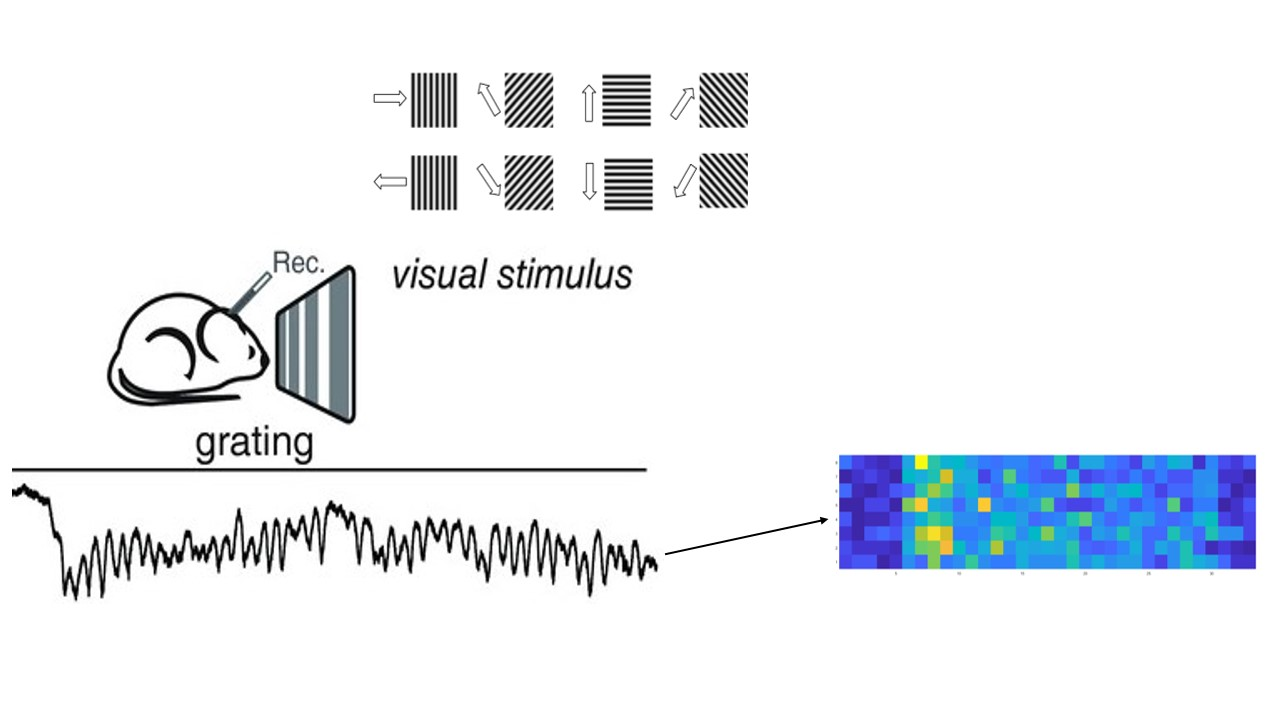
\includegraphics[width=0.55\textwidth]{figures/Slide5.jpg}
%             \caption{Visualising neural data from lab experiments.}
%     \end{figure}

% With this neural spiking data set, we can create  Each of the point cloud $X_i$ is thus represented by a matrix of dimension $698$-by-$264$, giving us a point cloud of $698$ points in $\RR^{264}$. 

% Our implementation  Using the (birth, death)-intervals from each persistence diagram, we drew the equivalent persistence barcode representation. The complete code can be found in Appendix \ref{AppendixA}. The following figures show the results from applying persistent homology.
% \begin{figure}[H]
% \centering
% \begin{subfigure}[b]{0.2\textwidth}
%     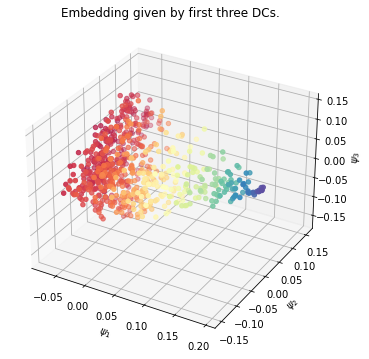
\includegraphics[width=\textwidth]{figures/X1_embedding.png}
%     \caption{Three-dimensional embedding of point cloud $X_1$.}
% \end{subfigure}
% \hfill
% \begin{subfigure}[b]{0.75\textwidth}
%     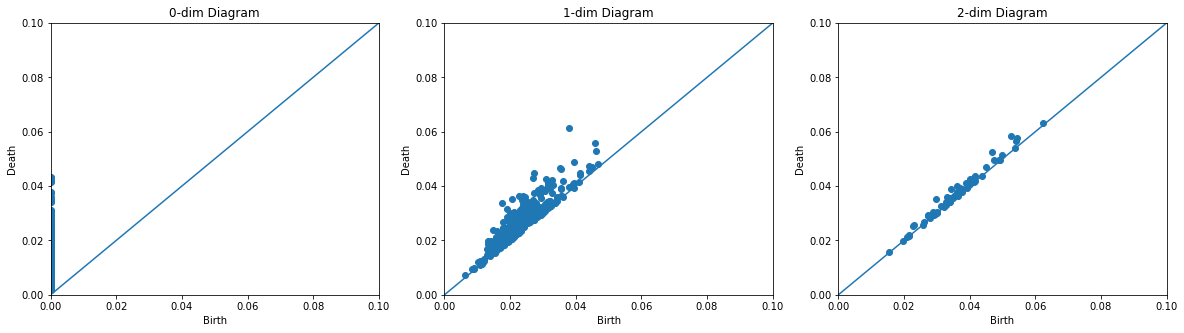
\includegraphics[width=\textwidth]{figures/X1_H0.png}
%     \caption*{Persistence diagrams.}
% \end{subfigure}
% \begin{subfigure}[b]{0.25\textwidth}
% 
\includegraphics[width=\textwidth]{figures/white.png} 
% \end{subfigure}
% \begin{subfigure}[b]{0.24\textwidth}
%     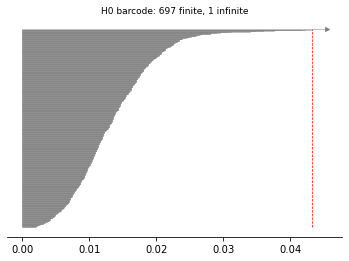
\includegraphics[width=\textwidth]{figures/X1_H0_barcode.png}
%     \captionsetup{labelformat=empty}
%     \caption{}
% \end{subfigure}
% \begin{subfigure}[b]{0.24\textwidth}
%     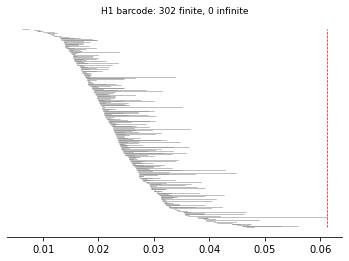
\includegraphics[width=\textwidth]{figures/X1_H1_barcode.png}
%         \caption*{Persistence barcodes.}
% \end{subfigure}
% \begin{subfigure}[b]{0.24\textwidth}
% 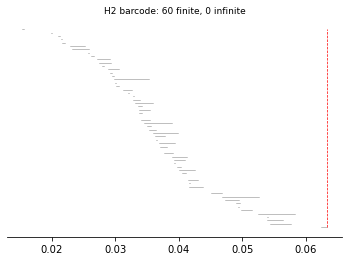
\includegraphics[width=\textwidth]{figures/X1_H2_barcode.png}
% \captionsetup{labelformat=empty}
%     \caption{}
% \end{subfigure}
% \caption{Results for applying persistent homology on the three-dimensional embedding of $X_1$.}
% \end{figure}
% Note that IEEE typically puts floats only at the top, even when this
% results in a large percentage of a column being occupied by floats.


% An example of a double column floating figure using two subfigures.
% (The subfig.sty package must be loaded for this to work.)
% The subfigure \label commands are set within each subfloat command, the
% \label for the overall figure must come after \caption.
% \hfil must be used as a separator to get equal spacing.
% The subfigure.sty package works much the same way, except \subfigure is
% used instead of \subfloat.
%
% \begin{figure*}[H]
% \centerline{\subfloat[Case I]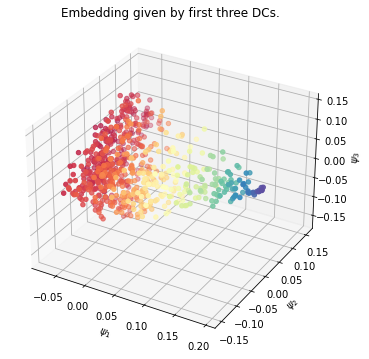
\includegraphics[width=2.5in]{figures/X1_embedding.png}\label{fig_first_case}}
% \hfill
% \subfloat[Case II]{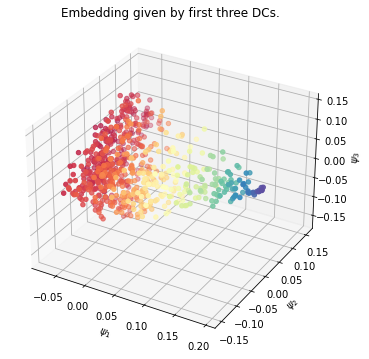
\includegraphics[width=2.5in]{figures/X1_embedding.png}\label{fig_second_case}}
% \caption{Simulation results}\label{fig_sim}
% \end{figure*}
%

% \begin{figure}[H]
%      \centering
%     \subfloat[][Experiments.]{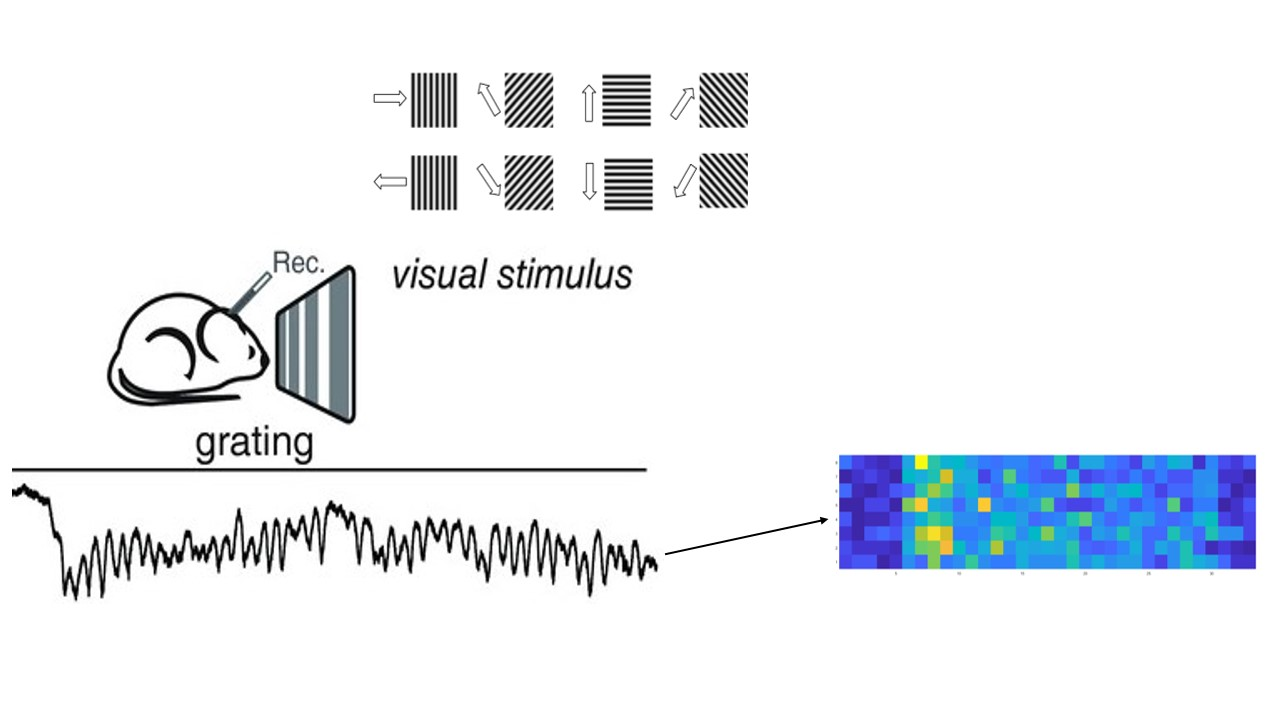
\includegraphics[width=0.6in]{figures/Slide5.jpg}\label{<figure1>}}
%      \subfloat[][Homology group $H_0$ for point cloud $X_1$. ]{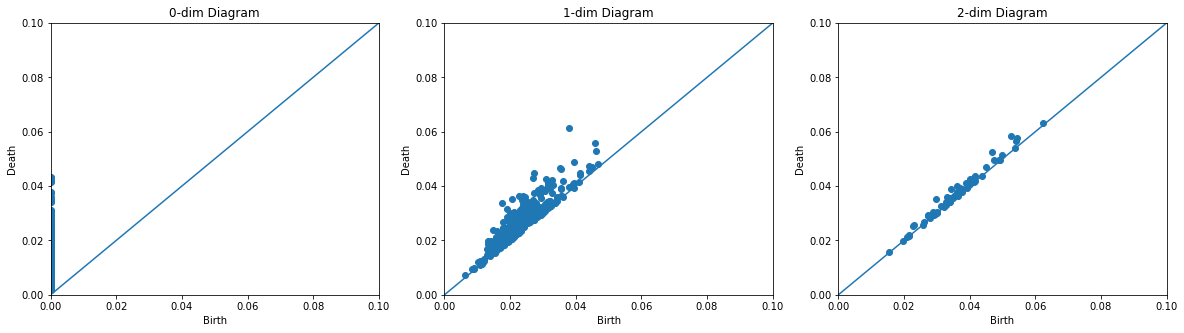
\includegraphics[width=2in]{figures/X1_H0.png}\label{<figure2>}}
     
%      \subfloat[][$X_1$.]{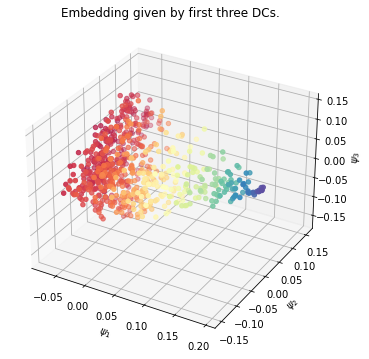
\includegraphics[width=0.6in]{figures/X1_embedding.png}\label{<figure1>}}
%      \subfloat[][Homology group $H_1$ for point cloud $X_1$. ]{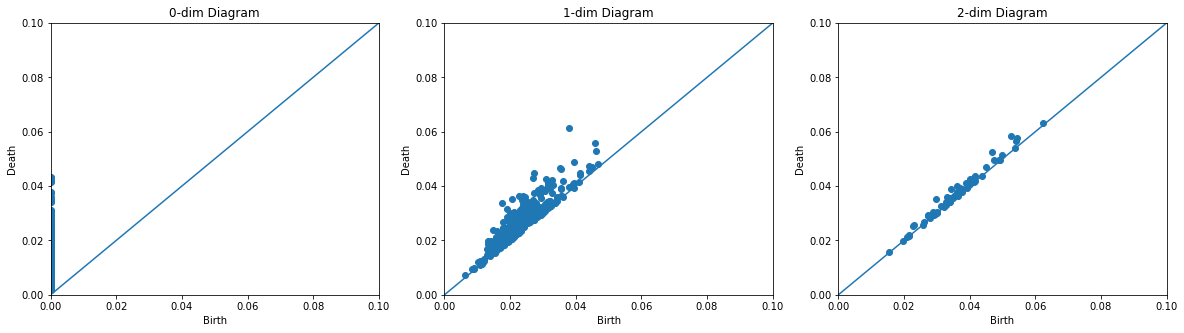
\includegraphics[width=2in]{figures/X1_H1.png}\label{<figure2>}}
%      \label{steady_state}
% \end{figure}

\begin{figure}[H]
\centering
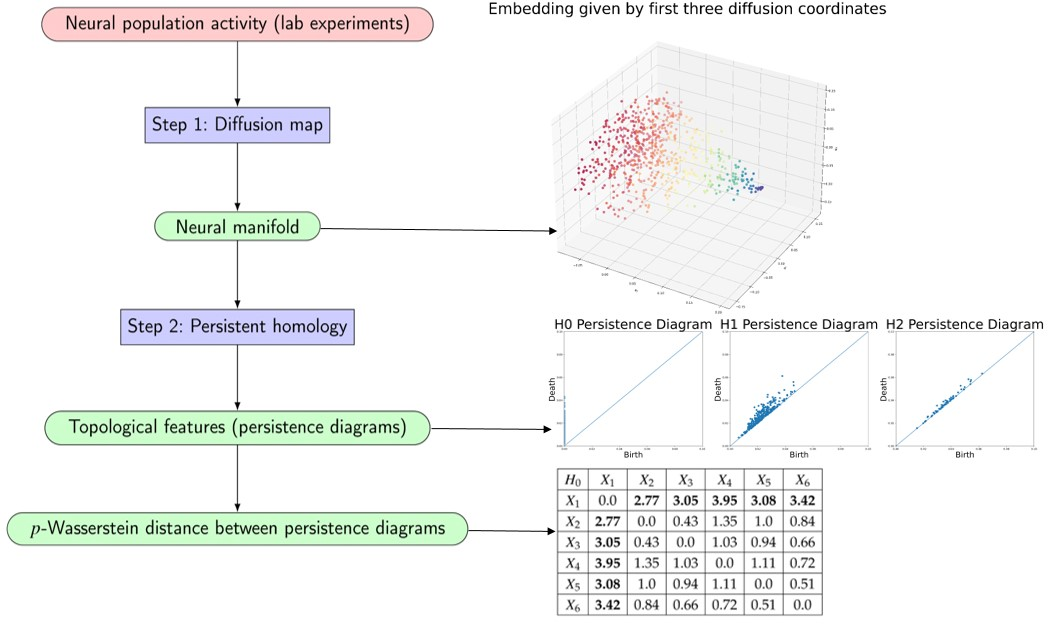
\includegraphics[width=5.5in]{flowchart.jpg}
\caption{Summary of the proposed approach and results.}
\label{fig_sim}
\end{figure}
% Note that often IEEE papers with subfigures do not employ subfigure
% captions (using the optional argument to \subfloat), but instead will
% reference/describe all of them (a), (b), etc., within the main caption.


% An example of a floating table. Note that, for IEEE style tables, the 
% \caption command should come BEFORE the table. Table text will default to
% \footnotesize as IEEE normally uses this smaller font for tables.
% The \label must come after \caption as always.
%
%\begin{table}[!t]
%% increase table row spacing, adjust to taste
%\renewcommand{\arraystretch}{1.3}
% if using array.sty, it might be a good idea to tweak the value of
% \extrarowheight as needed to properly center the text within the cells
%\caption{An Example of a Table}
%\label{table_example}
%\centering
%% Some packages, such as MDW tools, offer better commands for making tables
%% than the plain LaTeX2e tabular which is used here.
%\begin{tabular}{|c||c|}
%\hline
%One & Two\\
%\hline
%Three & Four\\
%\hline
%\end{tabular}
%\end{table}


% Note that IEEE does not put floats in the very first column - or typically
% anywhere on the first page for that matter. Also, in-text middle ("here")
% positioning is not used. Most IEEE journals/conferences use top floats
% exclusively. Note that, LaTeX2e, unlike IEEE journals/conferences, places
% footnotes above bottom floats. This can be corrected via the \fnbelowfloat
% command of the stfloats package.




% conference papers do not normally have an appendix


% use section* for acknowledgement

% trigger a \newpage just before the given reference
% number - used to balance the columns on the last page
% adjust value as needed - may need to be readjusted if
% the document is modified later
%\IEEEtriggeratref{8}
% The "triggered" command can be changed if desired:
%\IEEEtriggercmd{\enlargethispage{-5in}}

% references section

% can use a bibliography generated by BibTeX as a .bbl file
% BibTeX documentation can be easily obtained at:
% http://www.ctan.org/tex-archive/biblio/bibtex/contrib/doc/
% The IEEEtran BibTeX style support page is at:
% http://www.michaelshell.org/tex/ieeetran/bibtex/
%\bibliographystyle{IEEEtran}
% argument is your BibTeX string definitions and bibliography database(s)
%\bibliography{IEEEabrv,../bib/paper}
%
% <OR> manually copy in the resultant .bbl file
% set second argument of \begin to the number of references
% (used to reserve space for the reference number labels box)


% \begin{thebibliography}{1}

% \bibitem{SueYeon} \scriptsize
% SueYeon Chung and L F Abbott. “Neural population geometry: An approach for understanding biological and artificial neural networks”. In: Current Opinion in Neurobiology (2021)., 10.1016/j.conb.2021.10.010

% \bibitem{Carlsson}
% Carlsson, Gunnar (Jan. 2009). “Topology and data”. en. In: Bulletin of the American Mathematical Society 46.2, pp. 255–308. ISSN: 0273-0979. DOI: 10.1090/S0273- 0979- 09- 01249- X., 10.1090/S0273-0979-09-01249-X
% Singh, Gurjeet et al. (June 2008). “Topological analysis of population activity in visual cortex”. In: Journal of Vision 8.8, pp. 11–11. ISSN: 1534-7362. DOI: 10.1167/8.8.11., 10.1167/8.8.11

% \bibitem{Chaudhuri}
% Chaudhuri, Rishidev et al. (Sept. 2019). “The intrinsic attractor manifold and population dynamics of a canonical cognitive circuit across waking and sleep”. In: Nature Neuroscience 22.9, pp. 1512–1520. ISSN: 1546-1726. DOI: 10.1038/s41593-019-0460-x., 10.1038/s41593-019-0460-x

% \bibitem{Beshkov}
% Beshkov K, Tiesinga P. Geodesic-based distance reveals nonlinear topological features in neural activity from mouse visual cortex. Biol Cybern. 2022 Feb;116(1):53-68. doi: 10.1007/s00422-021-00906-5. Epub 2021 Nov 23. PMID: 34816322., 10.1007/s00422-021-00906-5

% \bibitem{Giusti}
% Giusti, Chad et al. (Nov. 2015). “Clique topology reveals intrinsic geometric structure in neural correlations”. en. In: Proceedings of the National Academy of Sciences 112.44, pp. 13455–13460. ISSN: 0027-8424, 1091-6490. DOI: 10.1073/pnas.1506407112., 10.1073/pnas.1506407112

% \bibitem{Bardin}
% Bardin, Jean-Baptiste, Gard Spreemann, and Kathryn Hess (Jan. 2019). “Topological exploration of artificial neuronal network dynamics”.en. In: Network Neuroscience 3.3, pp. 725–743. ISSN: 2472-1751. DOI: 10.1162/netn\_a\_00080., 10.1162/netn\_a\_00080

% \bibitem{Luciano}
% Luciano Dyballa et al. “Flow stimuli reveal ecologically appropriate responses in mouse visual cortex”. In: Proceedings of the National Academy of Sciences 115.44 (2018), pp. 11304–11309. DOI: 10.1073/pnas.1811265115., 10.1073/pnas.1811265115

% \bibitem{Mileyko}
% Mileyko, Yuriy, Sayan Mukherjee, and John Harer (2011). “Probability measures on the space of persistence diagrams”. In: Inverse Problems 27.12, p. 124007. DOI: 10.1088/0266-5611/27/12/124007

% \bibitem{Chazal1}
% Chazal, Frédéric and Bertrand Michel (Feb. 2021). “An introduction to Topological Data Analysis: fundamental and practical aspects for data scientists”. en. In: arXiv:1710.04019 [cs, math, stat]. arXiv: 1710.04019. URL: http://arxiv.org/abs/1710.04019 (visited on 10/17/2021).

% \bibitem{Chazal2}
% Chazal, Frédéric et al. (2009). “Proximity of persistence modules and their diagrams”. en. In: Proceedings of the 25th annual symposium on Computational geometry - SCG ’09. Aarhus, Denmark: ACM Press, p. 237. ISBN: 978-1-60558-501-7. DOI: 10.1145/1542362.1542407. URL: http: //portal.acm.org/citation.cfm?doid=1542362.1542407 (visited on 11/03/2021). Bibliography 45

% \bibitem{Coifman1}
% Coifman, R. R. et al. (2005). “Geometric diffusions as a tool for harmonic analysis and structure definition of data: Diffusion maps”. In: Proceedings of the National Academy of Sciences 102.21, pp. 7426–7431. ISSN: 0027-8424, 1091-6490. DOI: 10 . 1073 / pnas . 0500334102. URL: http : //www.pnas.org/cgi/doi/10.1073/pnas.0500334102 (visited on 08/05/2021).

% \bibitem{Coifman2}
% Coifman, Ronald R. and Stéphane Lafon (2006). “Diffusion maps”. In: Applied and Computational Harmonic Analysis 21.1, pp. 5–30. ISSN: 10635203. DOI: 10.1016/j.acha.2006.04.006. URL: https://linkinghub. elsevier.com/retrieve/pii/S1063520306000546 (visited on 08/05/2021).

% \bibitem{Eastman}
% Eastman, Peter et al. (2017). “OpenMM 7: Rapid development of high performance algorithms for molecular dynamics”. In: PLOS Computational Biology 13.7. DOI: 10.1371/journal.pcbi.1005659. 

% \bibitem{Edelsbrunner}
% Edelsbrunner, Letscher, and Zomorodian (Nov. 2002). “Topological Persistence and Simplification”. In: Discrete&Computational Geometry 28.4, pp. 511–533. ISSN: 1432-0444. DOI: 10.1007/s00454-002-2885-2. URL: https://doi.org/10.1007/s00454-002-2885-2.

% \bibitem{Kerber}
% Kerber, Michael, Dmitriy Morozov, and Arnur Nigmetov (June 2016). “Geometry Helps to Compare Persistence Diagrams”. en. In: arXiv:1606.03357 [cs]. arXiv: 1606.03357. URL: http://arxiv.org/abs/1606.03357 (visited on 10/01/2021).

% \bibitem{Singh}
% Singh, Gurjeet et al. (June 2008). “Topological analysis of population activity in visual cortex”. In: Journal of Vision 8.8, pp. 11–11. ISSN: 1534-7362. DOI: 10.1167/8.8.11. eprint: https://arvojournals.org/arvo/content\_public/journal/jov/933530/jov-8-8-11.pdf. URL:https://doi.org/10.1167/8.8.11.

% \bibitem{Stopfer}
% Stopfer, Mark, Vivek Jayaraman, and Gilles Laurent (Sept. 2003). “Intensity versus Identity Coding in an Olfactory System”. In: Neuron 39.6, pp. 991–1004. ISSN: 0896-6273. DOI: 10.1016/j.neuron.2003.08.011. URL: https : / / www . sciencedirect . com / science / article / pii / S089662730300535X.

% \bibitem{GUDHI}
% The GUDHI Project (2021). GUDHI User and Reference Manual. 3.4.1. GUDHI
% Editorial Board. URL: https://gudhi.inria.fr/python/latest/
% wasserstein\_distance\_user.html.

% \bibitem{Tralie}
% Tralie, Christopher, Nathaniel Saul, and Rann Bar-On (2018). “Ripser.py: A Lean Persistent Homology Library for Python”. In: The Journal of Bibliography 48 Open Source Software 3.29, p. 925. DOI: 10.21105/joss.00925. URL:https://doi.org/10.21105/joss.00925.

% \bibitem{Tsodyks}
% Tsodyks, Misha (Jan. 1999). “Attractor neural network models of spatial maps in hippocampus”. In: Hippocampus 9.4. Publisher: John Wiley & Sons, Ltd, pp. 481–489. ISSN: 1050-9631. DOI: 10.1002/(SICI)1098- 1063(1999)9:4<481::AID-HIPO14>3.0.CO;2-S. URL: https://doi. org/10.1002/(SICI)1098-1063(1999)9:4<481::AID-HIPO14>3.0.CO;2-S (visited on 11/02/2021).

% \bibitem{Zomorodian1}
% Zomorodian, Afra (2005a). “Computing Persistent Homology”. en. In:
% p. 15.

% \bibitem{Zomorodian2}
% Zomorodian, Afra J. (2005b). Topology for Computing. Cambridge University
% Press.

% \end{thebibliography}




% that's all folks
\end{document}


